\documentclass[a4paper,11pt]{article}

\usepackage{mathptmx}
\usepackage{amsmath}
\usepackage{setspace}
\usepackage{fancyhdr}
\usepackage{hyperref}
\usepackage[margin=0.59in]{geometry}
\usepackage{graphicx}
\usepackage{floatflt}
\usepackage{revnum}
\usepackage{float}
\usepackage{enumitem}
\usepackage[compact]{titlesec}
\usepackage{caption}
\usepackage{MnSymbol}

\captionsetup[figure]{font=footnotesize}

%%\renewcommand{\familydefault}{\sfdefault}
%\setcounter{page}{11}
% Set name
\newcommand{\jjm}[5]{\item {#1}: {``#2''}, {#3}, {#5}, (#4).}
\newcommand{\rs}{R. Saito}
\def\Gprime{{\rm G^{\prime}}}
\def\Gstar{\rm G^*}

\def\name{Eddwi Hesky Hasdeo}
\def\hes{{\bf E.~H. Hasdeo}}
\def\sub{\emph{submitted}}
\def\ip{\emph{in press}}
% Replace this with a link to your CV if you like, or set it empty
% (as in \def\footerlink{}) to remove the link in the footer:
\def\footerlink{}

% The following metadata will show up in the PDF properties
\hypersetup{
  colorlinks = true,
  urlcolor = blue,
  pdfauthor = {\name},
  pdfkeywords = {physics, carbon, nanotubes, hasdeo, eddwi, hesky},
  pdftitle = {\name: Curriculum Vitae},
  pdfsubject = {Curriculum Vitae},
  pdfpagemode = UseNone
}

\geometry{
  %body={6.7in, 9.2in},
  left=15mm,
  top=20mm,
  right=15mm,
  bottom=20mm
}

% Customize page headers
\pagestyle{fancy}
\lhead{\small{\it Eddwi Hesky HASDEO}}
\chead{}
\rhead{}
\lfoot{}
\cfoot{\thepage}
\rfoot{}
%% \pagestyle{myheadings}
%% \markright{\small{Hasdeo Part B2- Standard EF - CoMBIne2DFlat}}
%%\thispagestyle{empty}
%% \thispagestyle{fancy}
%% \lhead{}
%% \chead{}
%% \rhead{}
%% \lfoot{}
%% \cfoot{\thepage}
%% \rfoot{}

%%Custom section fonts
%\usepackage{sectsty}
\renewcommand{\familydefault}{\rmdefault}

%%\sectionfont{\rmfamily\mdseries\large}
%% \subsectionfont{\rmfamily\mdseries\itshape\large}

% Other possible font commands include:
% \ttfamily for teletype,
% \sffamily for sans serif,
% \bfseries for bold,
% \scshape for small caps,
% \normalsize, \large, \Large, \LARGE sizes.
% Make lists without bullets

\setlist{nosep}

\renewenvironment{itemize}{
  \begin{list}{}{
      \setlength{\leftmargin}{1.5em}
      \setlength{\parskip}{0pt}
      \setlength{\parsep}{0pt}
      \setlength{\itemsep}{3pt}
  }
}{
  \end{list}
}
% Don't indent paragraphs.
\setlength\parindent{0em}

%remove spacing
\setlength{\parskip}{0pt}
\setlength{\parsep}{0pt}

%\setlength{\headsep}{0pt}
\setlength{\topskip}{0pt}
%\setlength{\topmargin}{0pt}
%\setlength{\topsep}{0pt}
\setlength{\partopsep}{0pt}
\titlespacing{\section}{0pt}{0pt}{0pt}
\titleformat{\section}{\large\bfseries}{\thesection}{1em}{\scshape}
%\titleformat{\section}{\thesection}{1em}{\scshape}
%%\titlespacing*{\section}{0pt}{1.1\baselineskip}{\baselineskip}


\singlespacing
\begin{document}


% Place name at left
\section{Overview of Past Research}
\begin{figure}[h!]
\centering
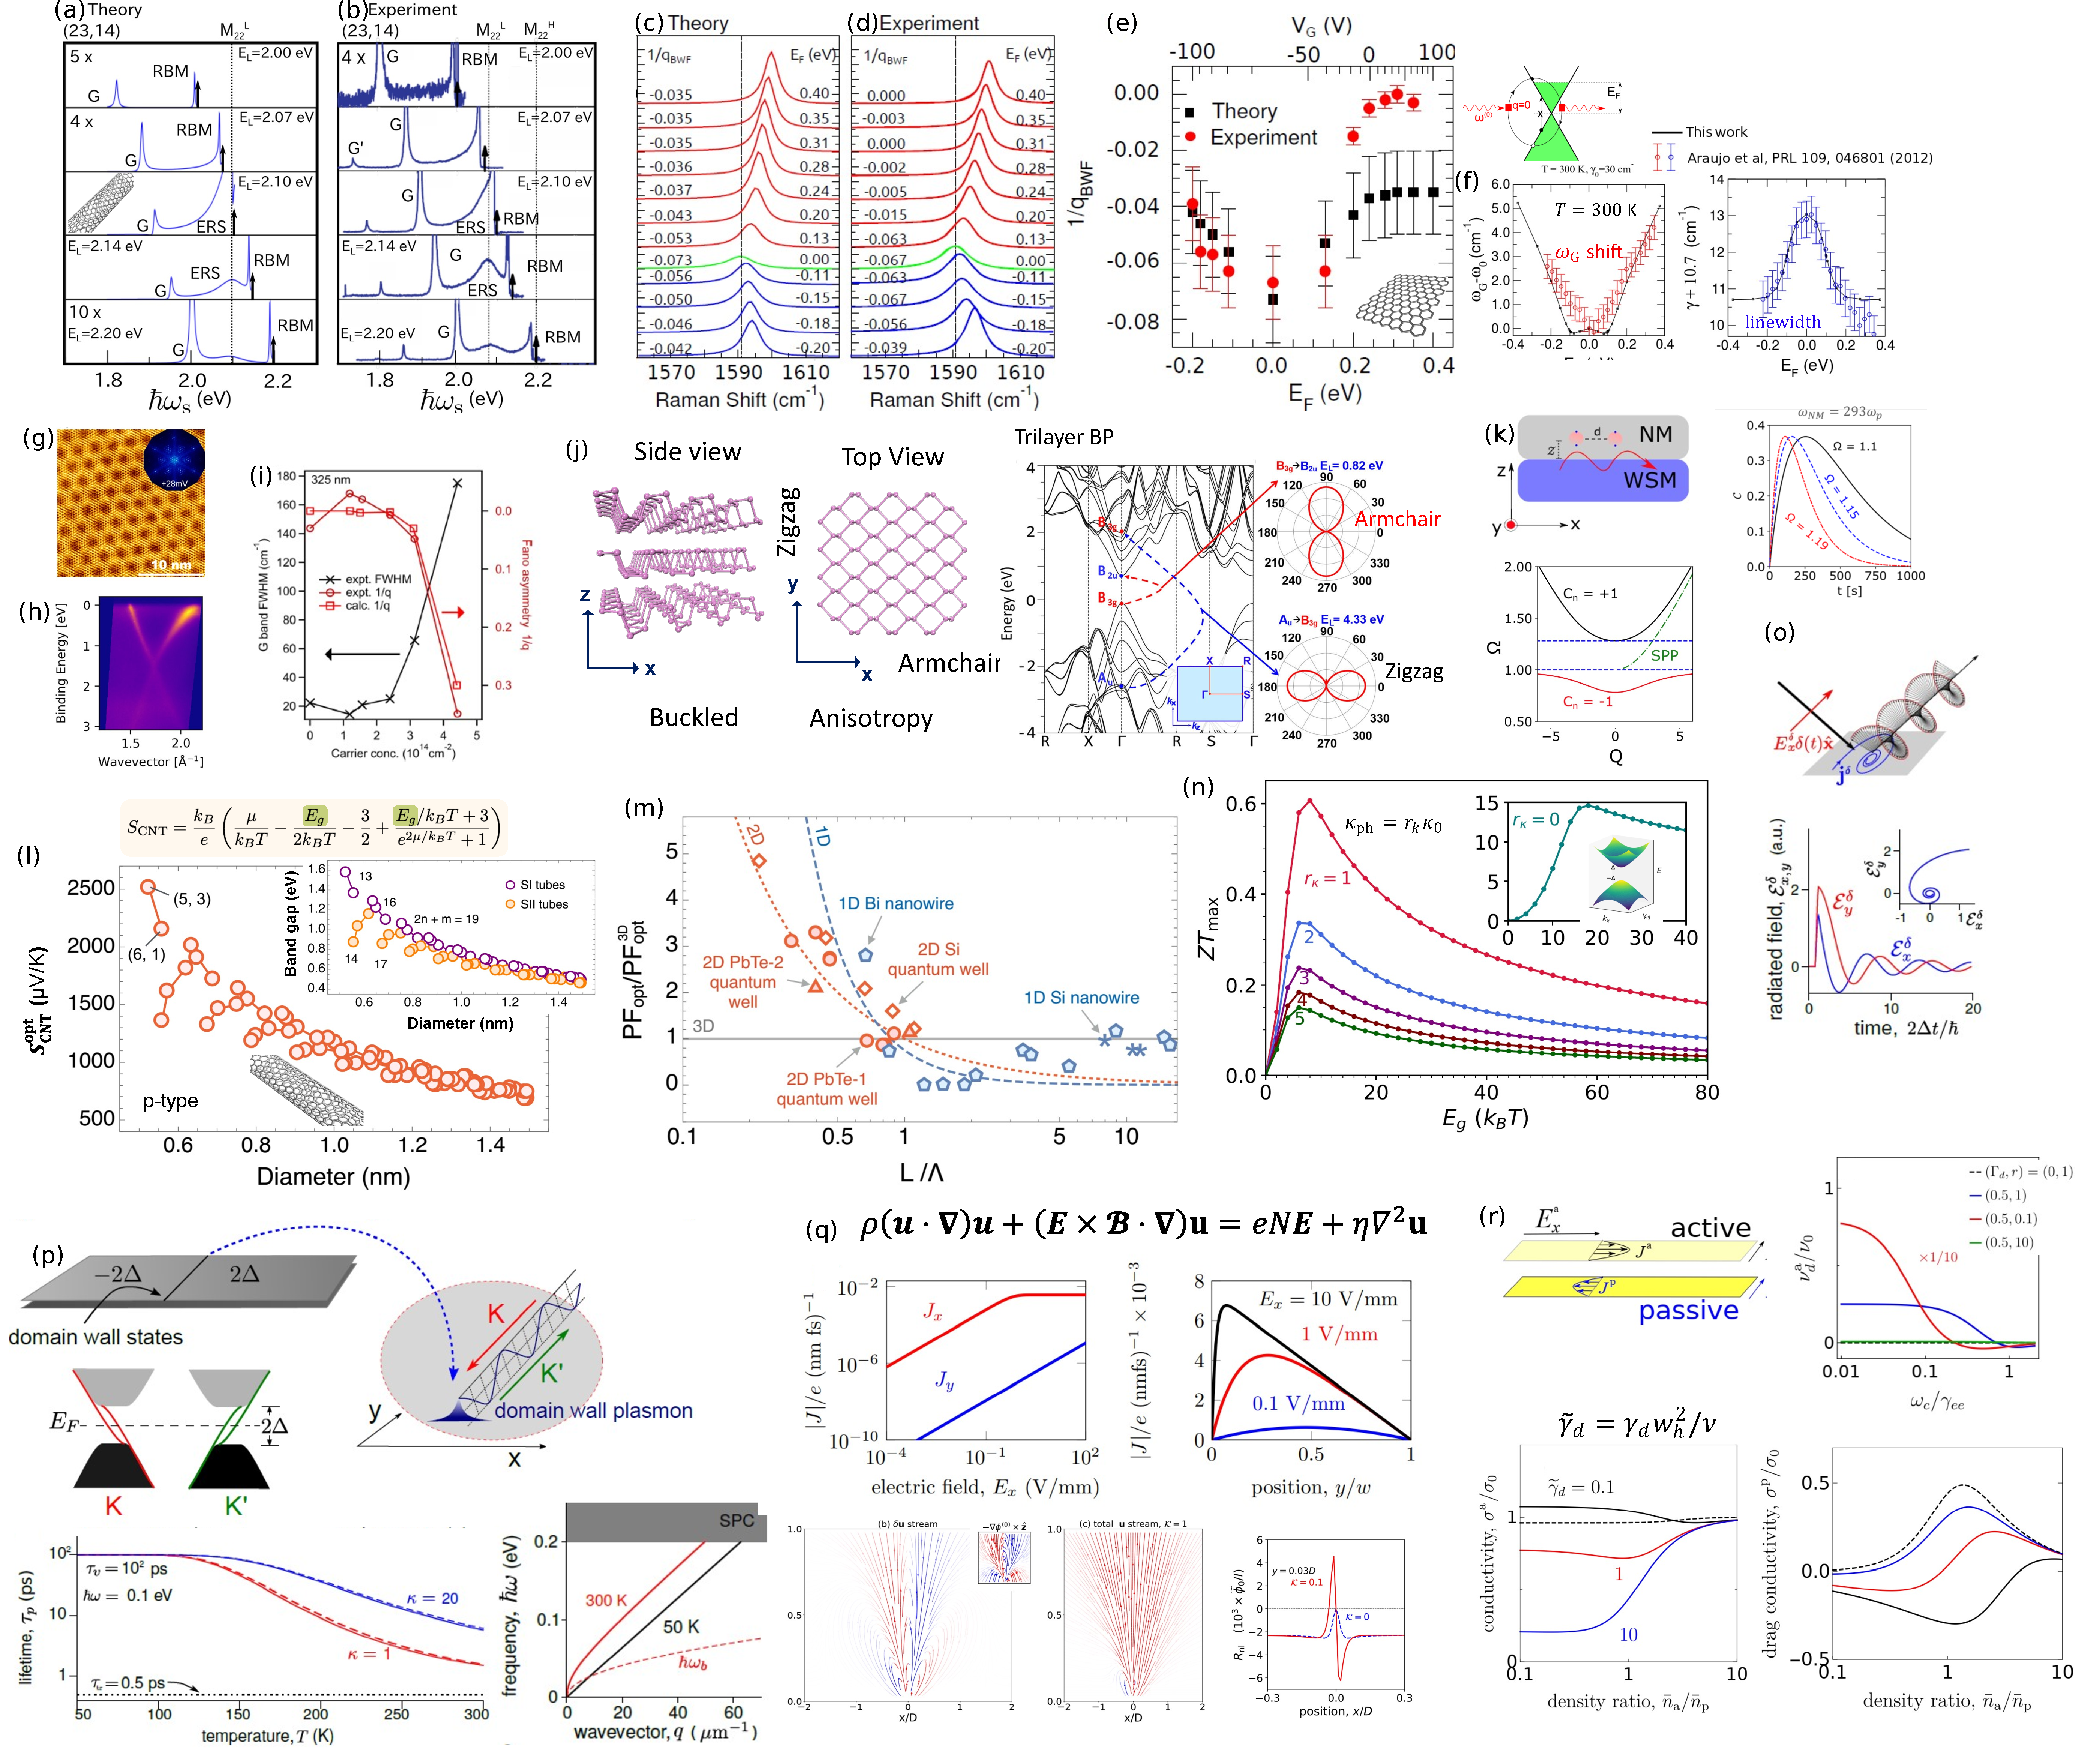
\includegraphics[width=18cm]{summary of past research}
\caption{{\bf Overview of past research}. (a)Electronic Raman spectra
  [PRB 88, 115107 (2013)]. Theoretical calculation of electronic Raman
  spectra (ERS) in metallic single wall nanotube (SWNT) for different
  laser energy $E_L$. Notice the ERS peak remains at electronic
  resonant energy $M_{22}^L$ and the G band spectra shows
  asymmetry. The calculation reproduces experiment (b). Raman shift
  $=E_L-\hbar \omega_s$ (c) Theoretical calculation of Raman spectra
  in graphene as a function of Fermi energy $E_F$ [PRB 90, 245140
    (2014)]. The Raman spectra exhibit Fano or Breit-Wigner-Fano
  asymmetry $1/q$ [see (e)] and change in peak position as well as
  linewidth [see (f)]. (d) Reproduce the experimental results. (e)
  Fano factor as a function of Fermi energy. (f) Kohn anomaly effect
  in graphene [PRB 94, 075104 (2016)]. Phonon self-energy calculation,
  the real part corresponds to frequency shift and the imaginary part
  is the inverse of lifetime. (g-i) Raman spectra of highly doped
  graphene [Nano Lett. 18, 6045(2018)]. (g) Scanning electron
  microscopy image of graphene on Ir (111). (h) Angle resolved
  photoemission spectroscopy of graphene under Cs doping. (i) G band
  linewidth and Fano asymmetry. The asymmetric factor is opposite from
  (e) because of Ir screening and first-order perturbation. (j)
  Anisotropic Raman spectra in black phosporous (BP) [Nano Lett. 16,
    2260 (2016)]. Buckled structure of BP allows detection of crystal
  orientation using photoabsorption and Raman spectra. (k) Topological
  photonics in Weyl semimetals (WSM) and uniaxial surface wave for
  qubit entanglement [PRB 106, 155409 (2022)]. Light inside WSM is
  topological with Chern number $\pm 1$. This gives rise to uniaxial
  surface wave [surface plasmon polariton (SPP) that can be used for
    qubit entanglement. The concurrence $\mathcal{C}$ measures the
    degree of entanglement that long last. (l) Diameter dependence of
    Seebeck coefficient (thermopower) in semiconducting SWNTs [PRB 92,
      165426 (2015)] to be compared with the bandgap. (m) Quantum
    enhancement of power factor of nanostructures [PRL 117, 036602
      (2016)] when $L/\Lambda<1$ where $L$ is the confinement length
    and $\Lambda$ is the thermal de Broglie wavelength. (n) Optimal
    band gap for thermoelectrics [JAP 126, 035109 (2019)]. $r_k$ is
    proportional to phonon thermal conductivity. (o) Detecting
    cyclotron motion without magnetic field [NJP 21, 083026
      (2019)]. Anomalous Hall materials exhibit cyclotron current that
    converts linear polarized pulse into circular polarized
    emission. (p) Plasmons of topological domain wall states in
    bilayer graphene [Nano Lett. 17, 7252 (2017)]. Plasmon of
    topological states transcend the bulk lifetime ($\tau_{\rm tr}\sim
    0.5$ ps) and limited by intervalley lifetime ($\tau_v$). The
    plasmon roperties are tunable by temperature and dielectric
    constant of substrate $\kappa$. (q) Quantum geometric correction
    to electronic Navier Stokes equation [PRB 103, 125106
      (2021)]. Here $\boldsymbol{\mathcal{B}}$ is proportional to the
    Berry flux in the Fermi surface. Including this term, we obtain
    asymmetric one-dimensional (1D) flow, back flow without boundary
    in 2D and asymmetric non-local resistance. (q) Negative drag in
    viscous fluid [PRB 107, L121107(2023)]. Drag conductivity can
    become negative in small channel width $W_h$. The negative drag is
    due to drag viscosity $\nu_d$ which is tunable by magnetic field,
    drag coefficient and density ratio. . }

\label{summary of past research}
\end{figure}

\subsection*{Raman spectroscopy of nanocarbons and two-dimensional materials}
Raman spectroscopy is inelastic scattering of light. Materials absorb
light (photon) energy and normally use it for atomic vibration (phonon
excitation). We studied a layer of carbon atoms that have the shape of a
honeycomb (graphene) and its allotrope rolled up into a single--wall carbon nanotube (SWNT).  Experiments in metallic SWNTs and
graphene showed a new Raman signal different from that of the phonon.  We
investigated this signal by developing programs to calculate electron
energy bands, phonon bands, electron-photon interactions,
electron-phonon interactions, and electron-electron interactions. We
explained the origin of electronic Raman signal and asymmetry in the
phonon band. We studied the renormalization of a phonon due to the conduction
electron --- Kohn anomaly and quantum interference effects observed in
Raman spectra. We extended the work into Raman spectra of black
phosphorous where we observed asymmetry in the electron photon and electron phonon.
\subsection*{Thermoelectric transport of low dimensional materials}
We were inspired by Hicks and Dresselhaus [PRB 47, 12727 (1993) \& 47,
  16631 (1993)] that low-dimensional materials might be good
thermoelectric materials. We jumped into the calculation of
thermoelectric properties of semiconducting SWNT and found diameter
dependence of thermopower similar to that of SWNT band gap energy. We then
develop a rule of thumb on how to obtain thermoelectric enhancement in
nanostructures, i.e. the confinement length should be smaller than the
thermal de Broglie wavelength. Furthermore, we model many kinds of
possible band structures to obtain high performance thermoelectric;
for exmple by looking at the optimized band gap, interplay with
topology, magnetism in CaMnO$_3$, and spin transport. 
\subsection*{Optoelectronics of quantum materials}
I realized that quantum materials hold great promise when a plethora of
new physics emerge. During my postdoctoral work in Singapore, I published two
papers on utilizing topological edge mode for long-lived plasmonics
and detecting cyclotron motion without magnetic field. The techniques
developed during my postdoctoral career have been pivotal for my career up to
now. This became an inspiration to the quantum hydrodynamic project, as
well as the detection of topological phase using rotation of optical
polarization (Faraday and Kerr effect). 
\subsection*{Hydrodynamic transport of quantum materials}
Among many two-dimensional (2D) materials, hexagonal
boron nitride turns out to be the perfect match for graphene as it
protects it from impurities. Graphene exhibits large mobility, and one
can imagine what transport may come out if we remove impurities and
leave the electrons with themselves. It turns out that the collective electron
moves like water obeying the hydrodynamic Navier-Stokes equation. We
develop hydrodynamic theory for quantum materials where the
wave function modifies electron motion which manifests in anomalous
velocity due to the Berry curvature. We obtained the quantum
correction to the Navier-Stokes equation and show asymmetric 1D flow
as well as unconventional back flow in 2D. In another project, we
consider a Coulomb drag mechanism in a bilayer viscous electron. We
discover a new drag viscosity due to interlayer interaction and show
that the drag conductivity can be negative in the limit of a small
channel. In the last project, we show how the spin-orbit coupling can
modify the electron viscosity. 
\subsection*{Topological quantum optics and qubits}
We are interested in contributing to the development of quantum computers
using quantum materials. We show that photons inside Weyl semimetal
are topological, which supports unidirectional surface waves --- surface
plasmon polaritons (SPP). This unique property is due to the breaking
of time-reversal symmetry that the Weyl semimetal possess. We utilize
this unidirectional SPP as a media to connect two quantum bits (qubits)
and show that the degree of entanglement can be kept for long times.
The other interest is to use the currently available quantum
computers as quantum simulators for manybody physics. We are at the
level of benchmarking and reproducing the previous results and will
utilize them in the systems with strong correlation.


\vspace*{\baselineskip}
\section{Research plan}

\begin{figure}[t]
\centering

\includegraphics[width=18cm]{researchplan}
\caption{{\bf Research plan:} Physical properties of quantum materials. [Topological systems] Van der Waals heterostructures such as graphene -- hexagonal boron nitride (hBN) or twisted bilayer
graphene exhibit the moir{\'e} pattern. This moir{\' e} potential
modifies the graphene band. We show band structure of 5 layer rhombohedral graphene on hBN that has flat bands and has recently been reported to show the fractional anomalous Hall effect [Nature, 626, 760 (2024)]. The other
example is for Weyl semimetals whose Berry curvature behaves like magnetic dipoles at two Weyl points. This can give rise to chiral anomaly effect, chiral magnetic effect, and axial-gravity anomaly. Topological insulators are bulk insulating states with dissipationless edge states. Here we take example of valley Hall states in inverted-gapped bilayer graphene. [Quantum geometry] Two aspects of quantum geometry manifest themselves in the Berry curvature and quantum metric. Berry curvature can be thought of as a self-rotating wave function that can give rise to transverse motion (anomalous
  Hall effect). The quantum metric appears when there exists a distance between the Bloch states $|\mathbf{k}\rangle$ and $|\mathbf{k+q}\rangle$. The wavefunctions consist of coherence superposition of multi-orbitals with different weights (mixed colors). Using optical and transport techniques, we will investigate the new response caused by quantum geometry. [Hydrodynamics of exotic phases] We will use hydrodynamic theory to describe spin-charge dynamics in strong spin-orbit systems or magnetic systems, conventional and exotic superconductors (e.g. anyon and topological superconductors)
  and anomalous Hall systems (Chern insulators) with integer or fractional quantized conductance, as well as quantum spin liquid where anti-ferromagnetic ordering in triangular lattice cause frustration. [Development of methods] Hydrodynamic transport can be
developed from the kinetic Boltzmann equation; this has been done in current research. In the future, we will incorporate the holography theory (AdS/CFT correspondence) where string theory and quantum gravity coincide. This theory corresponds to an ultra-strong correlation limit relevant to condensed matter systems without quasiparticles (e.g. high Tc superconducting cuprates). While all
theories mentioned above are developed using an effective analytic model
we also employ numerical method that runs on a quantum computer. For
the moment, this simulation is possible on one dimension only, and we will extend to a higher dimension.}
\end{figure}


\subsection*{Physical properties of quantum materials}
In the world of technologies built with quantum materials, computers
will be 100 times faster, electronics will be efficient and have
low energy consumption, energy generators will be cleaner and more
powerful, and energy storage will be lighter and have larger capacity.
Quantum materials are a new class of materials where quantum
mechanical wave functions govern the motion of electrons in a
nonclassical way or manifest in long-range order and
entanglement. The list of such materials relevant with the current
study includes topological insulators ---- insulating bulk with
dissipationless metallic surfaces, topological semimetals ---
electrons that obey the relativistic Dirac and Weyl equations,
superconductors, quantum spin liquid, integer, and fractional quantum
Hall states.

Quantum materials can be classified into two categories.  First, we
will study non-interacting systems with interesting structure of
wave functions (topology and quantum geometry). Second, the dynamics
of strongly correlated materials will be approached by hydrodynamic
theory as well as computation utilizing quantum computers.

\subsection*{a. Effect of quantum geometry in transport and optoelectronics}
The motion of electrons in a solid is governed by the energy dispersion
relations. The dispersion gives information of the kinetic energy as
well as how the particles respond to the external field. As quantum
particles, the structure of the wavefunction which emerges from
interaction with the periodic potential in solids provides an additional
non-classical ``driving force''. The so-called quantum geometry, which consists of the Berry curvature and quantum metric, is responsible for
the plethora of exotic transport observed in experiments. For example,
the quantum anomalous Hall effect, where electrons move with a
quantized conductance perpendicular to the applied electric field
($\mathbf{E}$) at zero magnetic field ($\mathbf{B}$) arises due to Berry's curvature [Science, 340, 167 (2013)]. The dramatic
contribution of the quantum metric is the observation of superconductivity
in flat bands in twisted bilayer graphene [PRL 131,240001
  (2023)]. Electrons in that system should have zero group velocity
and thus the wavefunction should be localized in space. However, the
quantum metrics dictate the size of the electron wavefunction and provide
additional ways for electrons to propagate.


{\bf Research purposes} Many new physics have been discovered in our
previous works including properties of collective electron waves
(plasmons) of topological edge states, unconventional electron flow in
topological materials, and unconventional linear and nonlinear
response in topological materials. All of those utilize the Berry
curvature as main source of non-classical ``driving force''. Now, we
will continue the project focusing on the quantum metric and its
interplay with the Berry curvature. We ask the following
questions. What is the optical and thermoelectric response in the
systems whose dynamics is governed by quantum metric? How to tune the
size of quantum geometry? We expect quantum geometry to emerge not
only in electronic bands but also in different platforms such as spin
waves, plasmons, phonons, and even classical waves. We will explore
all the possibilities.

{\bf Methods.} We start with the effective Hamiltonian whose bands obey the symmetry
that the quantum metric or Berry curvature will show up. From that
Hamiltonian, we derive the current operator non-perturbatively in the
presence of an electric field. We then collect the linear and non-linear
responses order by order. We expect that quantum metric will manifest
in the non-linear responses. We also derive the thermoelectric response in
the presence of electric field and temperature gradient. Normally, we
linearize the Boltzmann equation. We predict that we need to expand
the Boltzmann equation up to higher-order terms so that quantum metric may
come about in the electrical, thermoelectric and thermal
conductivities.  We extend this theory using realistic Hamiltonians
from tight binding or the first-principles calculation to assist
experimental efforts.

\subsection*{b. Hydrodynamic electrons in the exotic phase}

Recently, people have been fabricating graphene on top of substrates which have
strong spin-orbit coupling or magnetization. In the limit of very
clean samples, electrons should move according to the hydrodynamic
equation of motion. In the previous work, we showed that spin-orbit
coupling changes the electrons' viscosity. In the next project, we will
investigate the spin-relaxation of electrons, which is governed by the
electron-electron interaction. In hydrodynamics, the density, energy,
and momentum of fluids are conserved. In the spin-hydrodynamics, we
expect the conservation of spin--angular momentum which dictates the
kinematics of vortices in electron fluids. 

Hydrodynamics has been used as an effective description of strongly
correlated systems. For example, in the chiral fluid of quark-gluon
plasma, He$^4$ superfluids, and electrons at fractional quantum Hall
states.  Recently, multilayer rhombohedral graphene (mRG) on hexagonal
boron nitride (hBN) exhibits a fractional quantum Hall effect without
magnetic field. The fractional excitation is an indication of strong
correlation due to the flat band emerging from the moire potential induced
by the mRG-hBN lattice mismatch. The absence of the $\mathbf{B}$ field in this
phase describes the role played by quantum geometry. We will develop
the hydrodynamic theory of electrons in fractional quantum Hall states
by incorporating quantum geometry. Certain fractional states such as
$5/2$ are predicted to have non-trivial statistics different from
fermions (e.g. electrons) or bosons (e.g. photons) dubbed as
non-abelian anyons that is very important to the development of fault
tolerant quantum computers.

{\bf Research Purpose.} Hydrodynamic theory is relevant for describing strongly correlated
regimes where string theory and quantum gravity coincide. There are
several areas where this theory can be interesting, such as hydrodynamic
description of collective modes of non-abelian particles, measurement
of gravity and chiral anomaly --- violation of continuity relation due
to relativistic handedness --- outside the Weyl semimetals, and
transport of strongly correlated systems without Fermi surface.

{\bf Methods.} We develop the hydrodynamic equation from the kinetic Boltzmann
theory or from field theory with the imposing symmetry of the systems. The
first method requires detailed knowledge of quasiparticle
dispersion, quantum geometry, external field, and interactions. The
second method allows for universal description where the details do
not matter.

While hydrodynamic theory is a theory for large length and time
scales, we shall compare it with the numerical manybody problem. In
addition to the established numerical methods using classical
computers, we can utilize quantum circuits to simulate many-body dynamics. 

\subsection*{Ingenuity, importance and impact of this research}
We unravel the unchartered area to investigate the effects of quantum geometry
and strong correlation in optoelectronics. We are at the intersection
of quantum materials, photonics, and transport communities. Our
results are relevant to the development of quantum computers,
electronics, spintronics, valleytronics, photovoltaics,
thermoelectrics, and possibly new transport phenomena. We are
developing the theory using the state-of-the-art tools such as quantum
field theory, quantum geometry, and even quantum computers.






\section{Aspirations as an Inamori FP Faculty Member}
Under positive decision, I  aspire to
\begin{enumerate}
\item Secure competitive funding\\ I have experience to secure
  multi-years funding from domestic (Luxembourg or Indonesia),
  multilateral collaboration of two (Luxembourg and Germany) or three
  countries (e-Asia grant: Indonesia, Japan, and Thailand).  I will submit several proposals per year aiming to Kakenhi or international funding such as e-Asia.

\item Supervise graduate students and postdocs\\
With the secured grants, I will hire students and postdocs. I have experience in directing students even during my Ph.D. course. During one year or even less, we successfully published high-quality papers. These students successfully won the scholarship for their advanced study. There are three students currently doing PhD in Berkeley and some others in Korea, China, Singapore, and Japan thanks to the papers they published.
  In Luxembourg, I co-supervised 2 PhD students during my five-year stay.
\item Expand collaborative networks in Japan and internationally\\
I will promote the Institute of Advanced Studies, Kyushu University, through international conferences and collaborations. I have developed collaboration networks since my graduate course up to now. I connect with experimental and theoretical experts in Japan, Indonesia,
  Singapore, the Philippines, Thailand, Korea, Germany, Luxembourg,
  France, and America. Currently, I am a member of the Asia Pacific Center
for Theoretical Physics. I am planning to join thermoelectric and physics communities in Japan and internationally.
\end{enumerate}
\section{Research Achievements}

\subsection{Papers and other articles which have been published in academic journals   }
\subsubsection*{First-authored and corresponding authored papers}
\begin{enumerate}
\item E.G.~Idrisov$^\dagger$, \hes$^\dagger$, B.N.~Radhakrishnan, T.L.~Schmidt, ``Hydrodynamic Navier-Stokes equations in two-dimensional systems with Rashba spin-orbit coupling'', \href{https://doi.org/10.1063/10.0022364}{Low Temperature Physics 49, 1385-1397(2023)}.
\item J.M.~Adhidewata, R.W.M.~Komalig, M.S.~Ukhtary, A.R.T.~Nugraha, B.E.~Gunara, \hes, ``Trigonal warping effects on optical properties of anomalous Hall materials''\href{https://doi.org/10.1103/PhysRevB.107.155415}{Physical Review B 107, 155415 (2023)}.
\item \hes, E.G.~Idrisov, T.L.~Schmidt, ''Coulomb drag of viscous electron fluids: Drag viscosity and negative drag conductivity'', \href{https://doi.org/10.1103/PhysRevB.107.L121107}{Physical Review B 107 (12), L121107 (2023)}.
\item MS Muntini, E Suprayoga, SA Wella, I Fatimah, L Yuwana, T Seetawan, \hes, et al. ``Spin-tunable thermoelectric performance in monolayer chromium pnictides'', \href{https://doi.org/10.1103/PhysRevMaterials.6.064010}{Physical Review Materials 6 (6), 064010 (2022)}.
\item A Habibi, AZ Musthofa, E Adibi, J Ekström, TL Schmidt, \hes, ``Kerr and Faraday rotations in topological flat and dispersive band structures'',\href{https://iopscience.iop.org/article/10.1088/1367-2630/ac706d/meta}{New Journal of Physics 24 (6), 063003 (2022)}.
\item M Gaffar, SA Wella, \hes, `` Effects of topological band structure on thermoelectric transport of bismuthene'', \href{https://journals.aps.org/prb/abstract/10.1103/PhysRevB.104.205105}{Physical Review B 104 (20), 205105 (2021)}
\item E Suprayoga, WBK Putri, K Singsoog, S Paengson, MY Hanna, \hes, et al. ``Investigation of electron and phonon transport in Bi-doped CaMnO3 for thermoelectric applications'', \href{https://doi.org/10.1016/j.materresbull.2021.111359}{Materials Research Bulletin 141, 111359 (2021)}.
  \item \hes, J Ekström, EG Idrisov, TL Schmidt, ``Electron hydrodynamics of two-dimensional anomalous Hall materials'',\href{https://doi.org/10.1103/PhysRevB.103.125106}{Physical Review B 103 (12), 125106 (2021)}
  \item K.~Oktavian, \hes, ``Non-universal scaling of thermoelectric efficiency in 3D and 2D thermoelectric semiconductors'', \href{https://iopscience.iop.org/article/10.1088/2043-6262/abe93c/meta}{Advances in Natural Sciences: Nanoscience and Nanotechnology 12 (1), 015017 (2021)}.
\item B.~Rendy, \hes, ``Strain effects on band structures and Dirac nodal-line morphology of ZrSiSe'',\href{https://pubs.aip.org/aip/jap/article/129/1/014306/1065328}{ Journal of Applied Physics 129, 014306 (2021)}.
\item E.~Suprayoga, W.~B.~K Putri, K.~Singsoog, S.~Paengson, M.~Y.~Hanna, A.~R.~T.~Nugraha, D.~R.~Munazat, B.~Kurniawan, M.~Nurhuda, T.~Seetawan, \hes, ``Investigation of electron and phonon transport in Bi-doped CaMnO3 for thermoelectric applications'', \sub, \href{https://doi.org/10.1016/j.materresbull.2021.111359}{Mat. Res. Bul 141, 111359 (2021)}.
\item M.~Nurhuda, A.~R.~T. Nugraha, M.~Y. Hanna, E. Suprayoga, \hes, ``Thermoelectric properties of Mexican-hat band structures'', \href{https://doi.org/10.1088/2043-6254/ab7225}{Adv. Nat. Sci.: Nanosci. Nanotech., 11  015012 (2020)}
\item \hes, L. P. A. Krisna, B. E. Gunara, N. T. Hung, A. R. T. Nugraha: ``Optimal band gap for improved thermoelectric performance of two-dimensional Dirac materials'', \href{https://doi.org/10.1063/1.5100985}{Jour. Appl. Phys. 126, 035109 (2019)}.
\item \hes, A. J. Frenzel , J. C. W. Song: ''Cyclotron motion without magnetic field'',  \href{https://doi.org/10.1088/1367-2630/ab351c} {New J. Phys. 21, 083026 (2019)}.
  \item \hes,  and J. C. W. Song: ``Long-lived domain wall plasmons in gapped bilayer graphene'', \href{http://dx.doi.org/10.1021/acs.nanolett.7b02584}{Nano Lett. 17, 7252-7257 (2017)}.
\item \hes, A. R. T. Nugraha, M. Dresselhaus, R. Saito: `` Fermi
  energy dependence of first-and second-order Raman spectra in
  graphene: Kohn anomaly and quantum interference effect'',
  \href{http://dx.doi.org/10.1103/PhysRevB.94.075104}{ Phys. Rev. B 94, 075104 (2016)}.
 \item \hes, A. R. T. Nugraha, R. Saito, M. S. Dresselhaus:
    ``Breit-Wigner-Fano lineshapes in Raman spectra of graphene'',
    \href{http://dx.doi.org/10.1103/PhysRevB.90.245140} {Phys. Rev. B
      90, 245140 (2014)}.
    \item \hes,  A. R. T. Nugraha, K. Sato, R. Saito,
  M. S. Dresselhaus: ``Electronic Raman scattering and the Fano
  resonance in metallic carbon nanotubes'',
  \href{http://dx.doi.org/10.1103/PhysRevB.88.115107}{
      Phys. Rev. B 88, 115107 (2013)}.
\item \hes, M. Nurhuda, Abdurrouf: ``The Optical Low-Pass Filter Gain
  of a Ring Cavity'',
  \href{http://www.ijens.org/Vol_12_I_01/125701-9494-IJBAS-IJENS.pdf}
  {IJBAS-IJENS  01, 63-68 (2012)}.
\end{enumerate}

\subsubsection*{Other papers}
\begin{enumerate}
 \item E.P.~Sinaga, M.~Adams, M.~Bersweiler, L.G.~Vivas, \hes, et al.
   ``Micromagnetic simulation of neutron scattering from spherical nanoparticles: Effect of pore-type defects'',\href{https://doi.org/10.1103/PhysRevB.107.014416}{Physical Review B 107 (1), 014416 (2023)}
 \item JM Adhidewata, ART Nugraha, \hes, BE Gunara, ``Thermoelectrics of type-I and type-II nodal line semimetals within the two-band model'',\href{https://ijphysics.fi.itb.ac.id/index.php/ijp/article/download/326/307}{Indonesian Journal of Physics 33 (1), 51-57 (2022)}
   
 \item MS Ukhtary, \hes, AB Suksmono, ART Nugraha, ``Long-lived qubit entanglement by surface plasmon polaritons in a Weyl semimetal'',\href{https://doi.org/10.1103/PhysRevB.106.155409}{Physical Review B 106 (15), 155409 (2022)}

\item   JM Adhidewata, ART Nugraha, \hes, P Estellé, BE Gunara, ``Thermoelectric properties of semiconducting materials with parabolic and pudding-mold band structures'', \href{https://www.sciencedirect.com/science/article/pii/S2352492822005979}{Materials Today Communications 31, 103737(2022)}
\item J Ekström, \hes, MB Farias, TL Schmidt, `` Kerr effect in tilted nodal loop semimetals'', \href{https://doi.org/10.1103/PhysRevB.104.125411}{Physical Review B 104 (12), 125411 (2021)}

\item G. Suwito, M. Fukuda, E. Suprayoga, \hes, A. R. T. Nugraha, M. Sakashita, S. Shibayama, O. Nakatsuka, ``Formatio of ultra-thin $\rm Ge_{1-x}Sn_x/Ge_{1-x-y}Si_xSn_y$ quantum heterostructures and experimental observation of resonant tunneling phenomenon'', \href{https://doi.org/10.1063/5.0024905}{Appl. Phys. Lett. 117, 232104 (2020)}.
\item N. Ehlen, M. Hell, G. Marini, \hes, R. Saito, Y.~Falke, M.~O.~Goerbig, G. Di Santo, L. Petaccia, G. Profeta, A. Gruneis: ``Origin of the flat band in heavily Cs doped graphene'', \href{https://doi.org/10.1021/acsnano.9b08622}{ACS Nano 14, 1055 (2020)}.
  
  \item M. G. Hell, N. Ehlen, B. V. Senkovskiy, \hes, A. Fedorov† , D. Dombrowski, C. Busse, T. Michely, G. di Santo, L. Petaccia, R. Saito, and A. Gruneis: ''Resonance Raman Spectrum of Doped Epitaxial Graphene at the Lifshitz Transition'', \href{http://dx.doi.org/10.1021/acs.nanolett.8b02979}{Nano Letters, 18 (9), 6045 -- 6056 (2018) }.
\item Y. Harada, M. S. Ukhtary, M. Wang, S. K Srinivasan, \hes, A. R. T. Nugraha, G. T. Noe, Y. Sakai, R. Vajtai, P. M Ajayan, R. Saito, J. Kono: ``Giant Terahertz-Wave Absorption by Monolayer Graphene in a Total Internal Reflection Geometry'', \href{http://dx.doi.org/10.1021/acsphotonics.6b00663} {ACS Photonics  4 121 (2017)}.
\item A. R. T. Nugraha, \hes, R. Saito: ``Selective coherent phonon mode generation in single-wall carbon nanotubes'', \href{
https://dx.doi.org/10.1088/1361-648X/29/5/055302}{Jour. Phys. Cond. Matt. 29, 055302 (2017)}.
\item D. Zhang, J. Yang, \hes, C. Liu, K. Liu, R. Saito, Y. Li:
  ``Multiple Electronic Raman Scatterings in a Single Metallic Carbon
  Nanotube'',
  \href{http://dx.doi.org/10.1103/PhysRevB.93.245428}{Phys. Rev. B 93,
    245428 (2016)}.
\item N. T. Hung, \hes, A. R. T. Nugraha, M.  Dresselhaus, R. Saito:
  ``Quantum effects on thermoelectric power factor of low-dimensional
  semiconductors'', \href{http://dx.doi.org/10.1103/PhysRevLett.117.036602}{Phys. Rev. Lett. 117, 036602 (2016)}.

\item M. S. Ukhtary, A. R. T. Nugraha, \hes, R. Saito: ``Broadband
  Transverse Electric Surface Wave in Silicene'',
  \href{http://dx.doi.org/10.1063/1.4960531}{Appl. Phys. Lett. 109,
    063103 (2016)}.
\item X. Ling, S. Huang, \hes, L. Liang, W. M. Parkin, Y. Tatsumi,
  A. R. T. Nugraha, A. A. Puretzky, P. M. Das, B. G. Sumpter,
  D. B. Geohegan, J. Kong, R. Saito, M. Drndic, V. Meunier,
  M. S. Dresselhaus: ``Anisotropic Electron-Photon and Electron-Phonon
  Interactions in Black Phosphorus'',
  \href{http://dx.doi.org/10.1021/acs.nanolett.5b04540} {Nano Lett.,
    16, 2260 (2016)}.
\item P. Ayria, A. R. T. Nugraha, \hes, T. R. Czank, S. Tanaka, R. Saito:
``Photon energy dependence of angle-resolved photoemission spectroscopy in graphene'', \href{http://dx.doi.org/10.1103/PhysRevB.92.195148} {Phys. Rev. B 92, 195148 (2015)}. 
\item N. T. Hung, A. R. T. Nugraha, \hes, M. S. Dresselhaus, R. Saito:
  ``Diameter dependence of thermoelectric power of semiconducting
  carbon nanotubes'', \href{http://dx.doi.org/10.1103/PhysRevB.92.165426}
  {Phys. Rev. B 92, 165426 (2015)}.
\item R. Saito, A. R. T. Nugraha, \hes, S. Siregar, H. Guo, T. Yang:
  ``Ultraviolet Raman spectroscopy of graphene and transition-metal
  dichalcogenides'', \href{http://dx.doi.org/10.1002/pssb.201552201}
  {Phys. Status Solidi B 252, 2363 (2015)}.
\item M. S. Ukhtary, \hes, A. R. T. Nugraha, R. Saito: ``Fermi
  energy-dependence of electromagnetic wave absorption in graphene'',
  \href{http://dx.doi.org/10.7567/APEX.8.055102} {APEX 8, 055102 -1-4,
    (2015)}. 
\item A. R. T. Nugraha, \hes, G. D. Sanders, C. J. Stanton, R. Saito:
  ``Origin of coherent G-band phonon spectra in single wall carbon
  nanotubes'', \href{http://dx.doi.org/10.1103/PhysRevB.91.045406}
  {Phys. Rev. B 91, 045406 (2015)}.  

  \item H.-L. Liu, S. Siregar, \hes, Y. Kumamoto, C.-C. Shen,
    C.-C. Cheng, L.-J. Li, R. Saito, S. Kawata: ''Deep-ultraviolet
    Raman scattering studies of monolayer graphene thin films'',
    \href{http://dx.doi.org/j.carbon.2014.10.028}{Carbon 81, 807-813
      (2015)}.
\item A. R. T. Nugraha, E. Rosenthal, \hes,
  G. D. Sanders C. J. Stanton, M. S. Dresselhaus, R. Saito:
  ``Excitonic effects on coherent phonon dynamics in single wall
  carbon nanotubes'',
  \href{http://dx.doi.org/10.1103/PhysRevB.88.075440}{ Phys.
      Rev. B 88, 075440 (2013)}.
\end{enumerate}
 \vspace*{\baselineskip}
\subsubsection*{Book Chapter}
\begin{enumerate}
\item R. Saito, A. R. T. Nugraha, \hes, N. T. Hung, W. Izumida (2017), ``Electronic and Optical Properties of Single Wall Carbon Nanotubes'', Topics in Current Chemistry, 375, 7 (2017), Springer, ISSN: 2365-0869 (Print) \href{http://dx.doi.org/10.1007/s41061-016-0095-2}{2364-8961 (Online)}.
\end{enumerate}

\vspace*{\baselineskip}

\subsubsection*{Proceedings}
\begin{enumerate}
 \item E Suprayoga, MY Hanna, \hes, ART Nugraha,
   ``A comparative study of thermoelectric properties of monolayer, bilayer and bulk CrI$_3$'', \href{https://doi.org/10.1063/5.0059994}{AIP Conference Proceedings 2382 (2021)}.
\item NR Ayukaryana, MH Fauzi, \hes, ``The quest and hope of Majorana zero modes in topological superconductor for fault-tolerant quantum computing: An introductory overview'', \href{https://doi.org/10.1063/5.0059974}{AIP Conference Proceedings 2382 (2021)}.
 \item \hes, L. Krisna, A. R. T. Nugraha:
  ``Thermoelectric properties of two-dimensional Dirac materials'',
   \href{https://doi.org/10.1063/5.0014592} {AIP Conf. Proc 2256, 030010 (2020)}.
\item E. Suprayoga, A. Rifai, A. Subhan, G. K. Sunardinanto, M. Y. Hanna, \hes,  A. R. T. Nugraha: ``Ab-initio calculation of muon spin polarization function to study lithium-ion diffusion in $\rm LiTi_2O_4$ battery material'', \href{https://doi.org/10.1063/5.0014693}{AIP Conf. Proc. 2256, 030015 (2020)}. 
\item A. R. T. Nugraha, M. Y. Hanna, E. Suprayoga, \hes: ``Modulation of coherent phonon amplitudes in low-dimensional materials by ultrafast laser pulse trains'', \href{https://doi.org/10.1063/5.0023505}{AIP Conf. Proc. 2256, 020005 (2020)}.
\item M. Y. Hanna, \hes, E. Suprayoga and A. R. T. Nugraha: ``Thermoelectric properties of two-dimensional hydrogenated borophene: A first-principles study'', \href{https://doi.org/10.1063/5.0014610}{AIP Conf. Proc. 2256, 030017 (2020)}
\item A. R. T. Nugraha and \hes: ``Coherent and squeezed phonons in single wall carbon nanotubes'', \href{https://doi.org/10.1088%2F1742-6596%2F1191%2F1%2F012002}
{Jour. Phys. Conf. Ser. 1191, 012002 (2019)}.
\end{enumerate}
\vspace*{\baselineskip}

\subsection{Presentations at international conferences and symposiums}
\subsubsection*{Oral Presentation}
\begin{enumerate}
  \jjm{\hes} {Effects of electron wave function in optoelectronics and
    transport} {International Symposium on Physics and Applications}
      {2023.11.21 --22}{ITS Surabaya, Indonesia }$\medstar$
\jjm{ T
        Schmidt, \hes $\bigcirc$, E Idrisov} {Coulomb drag of viscous
        electron fluids: drag viscosity and negative drag
        conductivity} {APS March Meeting} {2023.03. 5--10}{ Las Vegas,
        USA}
\jjm{\hes}{Negative drag conductivity in viscous electrons}{National Physics Seminar}{2022.08.27 }{Unesa Surabaya }$\medstar$

\jjm {\hes $\bigcirc$, MS Ukhtary, ART Nugraha, AB Suksmono}
     {Topological photonics and unidirectional surface plasmon polaritons in a Weyl semimetals}{APS March Meeting}
     {2023.03. 05--10}{ Las Vegas, USA}
     \jjm {P Poduval, T Schmidt, \hes}
          {Plasmon-induced magnetization in the edges of higher Chern insulators}{APS March Meeting}
          {2022}{Online}
          \jjm{\hes $\bigcirc$, E Idrisov, T Schmidt}
              {Electron-hole drag viscosity and magnetotransport in semimetals}
              {APS March Meeting}
              {2022}
              {Online}
              \jjm{E Sinaga, L Vivas, \hes, P Bender, A Michels}
                  {Magnetic neutron scattering of nanoparticles: failure of the superspin model}{APS March Meeting}
              {2022}
              {Online}
              \jjm{\hes$\bigcirc$, E Idrisov, J Ekstr{\"o}m, T Schmidt}{Navier-Stokes flows meet topological electronics}{APS March Meeting}
              {2022}
              {Online}
\jjm{\hes}
{Hydrodynamic transport and optical properties of anomalous Hall materials}
{The 11$^{\rm th}$ International Conference on Theoretical and Applied Physics}
{2021.10.27 -- 28}
{Unair, Surabaya}$\medstar$

\jjm{A Habibi, J Ekstr{\"o}m, T Schmidt, \hes $\bigcirc$}{Kerr and Faraday rotations of two dimensional topological flat bands}{Deutsche Physikalische Gesellschaft}{2021. 9.27 -- 10.1}{Online}
  \item \hes: ``Novel Optoelectronics of Nanomaterials'', Brawijaya University, Physics Departmental Seminar, (26/12/2018)$\medstar$
  \item \hes: ``Theoretical analysis of quantum materials for optoelectronics'', Bandung Institute of Technology, Physics Departmental Seminar, (23/11/2018) $\medstar$
  \item \hes: ``Optoelectronics of low dimensional materials'', University of Indonesia, Physics Departmental Seminar, (12/09/2018)$\medstar$
  \item \hes, J. C. W. Song: “Novel plasmonics in topological edge states of gapped bilayer graphene”, NUS, Physics Departmental Seminar, Singapore, (30/08/2017)$\medstar$

% India-Japan Seminar JSPS 2014
% 
\jjm{\rs, \hes, K. Sato, S. Siregaar, H. H. Guo, T. Yang}
{Raman spectroscopy of graphene and transition metal dichalcogenides atomic layer (invited)}
{Physics and Chemistry of Atomic Films: Fundamental Science and Applications}
{2014.11.4-8}{Jawaharlal Nehru Centre for Advanced Scientific
  Research, Bangalore, India}
\jjm{Ahmad R. T. Nugraha, \hes, \rs} %#Oral 2-11
{Coherent and squeezed phonons in single wall carbon nanotubes}
{The 48th Fullerenes-Nanotubes-Graphene General Symposium}
{2015.2.21-23}{The University of Tokyo}

% Kirchberg winterschool 2015
\jjm{\rs, \hes, A. R. T. Nugraha, H. Guo, T. Yang, S. Siregar}
{Raman spectroscopy of graphene and transition metal dichalcogenides (invited)}
{29th International Winterschool on Electronic Properties of Novel Materials: ``Molecular nanostructures''}
{2015.3.7-14}{Kirchberg, Austria}

% NT15 
%2015 CCTN15, #Contributed Talk
\jjm{\hes$\circ$, A. R. T. Nugraha, \rs} {Interplay of
  electron-phonon and electron-electron interactions in gate modulated
  Raman spectroscopy of graphene} {CCTN15: The Tenth International
  Symposium on Computational Challenges and Tools for Nanotubes}
{2015.06.28}{Nagoya University, Japan}
\jjm{\rs, M. S. Ukhtary, \hes, A. R. T. Nugraha, C. Reynolds}
{Tunable absorption of electromagnetic wave at graphene interface between two dieletcric materials (invited)}
{6th RIEC-RLE meeting on research collaboration in photonics}
{2015.10.26}{Sendai}
% A3
\jjm{\rs, Y. Tatsumi, A. R. T. Nugraha, \hes, H. L. Liu, H. Guo, T. Yang}
{Raman spectra of transition metal dichalcogenides and phosphorene (invited)}
{6th A3 symposium on Emerging Materials, Kyushu University}
{2015.11.9-11}
{Fukuoka}
% Riken Topical meeting
\jjm{\rs, M. S. Uktahry, A. R. T. Nugraha, \hes, C. Reynolds}
{Tunable absorption of electromagnetic wave of graphene (invited)}
{CEMS Topical meeting on Emergent 2D Materials}
{2015.12.12}{Riken, Wako}
    
\jjm{A. R. T. Nugraha, \hes, \rs}
{Coherent phonon spectra of G band in single wall carbon nanotubes}
{NT14: The Fifteenth International Conference on the Science and Application of Nanotubes}
{2014.06.02-06}{University of Southern California, Los Angeles, USA}
%2014 NT14, #T2
\jjm{\hes, A. R. T. Nugraha, M. S. Dresselhaus, \rs}
{Quantum interference effect in Raman spectra of metallic nanotubes}
{NT14: The Fifteenth International Conference on the Science and Application of Nanotubes}
{2014.06.02-06}{University of Southern California, Los Angeles, USA}
%2014.6.11 RIEC symposium
\jjm{\rs, \hes, K. Sato, H. H. Guo}
{Raman spectroscopy of graphene and atomic layer materials (invited)}
{RIEC symposium on Graphene}
{2014.6.11}{Tohoku University}

%2014 Zao14
\jjm{A. R. T. Nugraha, \hes, \rs, G. D. Sanders, C. Stanton}
{Coherent G band phonons in single wall carbon nanotubes}
{ATI 2014 Nano-Carbon Meeting}
{2014.7.31-8.1}{Yamagata-Zao}

%2014 Zao14
\jjm{ \hes, A. R. T. Nugraha, \rs}
{Asymmetric lineshape in G band Raman spectra of graphene}
{ATI 2014 Nano-Carbon Meeting}
{2014.7.31-8.1}{Yamagata-Zao}
%MRS-id Meeting 2014
%September 28, 13:25-13:50
\jjm{\rs, A. R. T. Nugraha, \hes, S. Siregar, M. S. Ukhtary}
{Raman and coherent phonon spectroscopy of carbon nanotubes and graphene (invited)}
{Materials Research Society of Indonesia Meeting 2014}
{2014.9.26-28}{Aston Denpasar Hotel and Convention Center, Bali, Indonesia}

%September 28, 13:50-14:05
\jjm{A. R. T. Nugraha, \hes, \rs}
{Origin of coherent phonons in single wall carbon nanotubes}
{Materials Research Society of Indonesia Meeting 2014}
{2014.9.26-28}{Aston Denpasar Hotel and Convention Center, Bali, Indonesia}
\jjm{\rs, \hes, S. Siregar, H. Guo, T. Yang} 
{Raman spectra of Graphene and transition metal dichalcogenides (invited)}
{The 5th A3 Symposium on Emerging Materials}
{2014.10.19-21}{Nankai University, China}
%2013 FNTG 44, #3-8
\jjm{A. R. T. Nugraha, \hes, \rs}
{Exciton effects on coherent phonon spectroscopy of carbon nanotubes}
{The 44th Fullerenes-Nanotubes-Graphene General Symposium}
{2013.03.11-13}{The University of Tokyo}
\jjm{\rs, A. R. T. Nugraha, \hes, K. Sato}
{Raman spectroscopy of metallic single wall nanotubes and doped graphene (invited)}
{4th A3 Symposium on Emerging Materials: Nanomaterials for Energy and
Electronics}
{2013.11.10-14}{Daemyung Resort, Jeju, Korea}
% Regensburg Invitation with air ticket
%
\jjm{\rs, K. Sato, \hes, A. R. T. Nugraha}
{Coherent phonon and Raman spectroscopy of single wall carbon nanotubes (invited)}
{Building blocks for carbon-based electronics: from molecules to nanotubes}
{2013.4.10-12}{University of Regensburg}
% Wonton 2013 Santa fe 
%
\jjm{\rs, \hes, A. R. T. Nugraha}
{Exciton effects on coherent phonon and electronic Raman spectroscopy of 
single wall carbon nanotubes (invited)}
{5th Workshop on Nanotube Optics and Nanospectroscopy}
{2013.6.16-20}{Eldorado Hotel, Santa Fe, NM, USA}

\end{enumerate}
\subsection*{Poster Presentations}
\begin{enumerate}
  \jjm{\hes $\bigcirc$, E Idrisov, T Schmidt}
      {Electron hydrodynamics in quantum materials}
      {ICTP summer school}
      {2023.09.22--30}{Bukhara, Uzbekistan}
\jjm{\hes, Ahmad R. T. Nugraha, \rs} 
{Kohn anomaly and quantum interference of one- and two-phonon
Raman spectra in graphene}
{NT16: The Seventeenth International Conference on the Science and Application of
  Nanotubes and Low-dimensional Materials}
{2016.8.7-13}{University of Vienna, Austria}
\jjm{\hes, Ahmad R. T. Nugraha, \rs} 
{Asymmetric Kohn anomaly in $\Gprime$ band of graphene}
{The 50th Fullerenes-Nanotubes-Graphene General Symposium}
{2016.2.20-22}{The University of Tokyo}

%2013 FNTG 44, #3P-19
\jjm{\hes, A. R. T. Nugraha, K. Sato, \rs}
{Electronic Raman scattering and origin of the Fano resonance in metallic carbon nanotubes}
{The 44th Fullerenes-Nanotubes-Graphene General Symposium}
{2013.03.11-13}{The University of Tokyo}
% NT13 (poster)
%
\jjm{A. R. T. Nugraha, \hes, \rs}
{Coherent phonons and single phonon mode generation in carbon nanotubes}
{6th A3 symposium on Emerging Materials}
{2015.11.9-11}{Kyushu University, Fukuoka}
\jjm{\hes, A. R. T. Nugraha, \rs}
{Screening of electron-phonon coupling due to electron-electron interaction in graphene}
{6th A3 symposium on Emerging Materials}
{2015.11.9-11}{Kyushu University, Fukuoka}
% P-2
\jjm{M. S. Ukhtary, \hes, A. R. T. Nugraha, \rs}
{Switching of electromagnetic wave by graphene}
{NT15: The Sixteenth International Conference on the Science and Application of Nanotubes}
{2015.06.29-07.03}{Nagoya University, Japan}

\jjm{A. R. T. Nugraha, \hes, \rs}
{Squeezed phonons in single wall carbon nanotubes}
{NT15: The Sixteenth International Conference on the Science and Application of Nanotubes}
{2015.06.29-07.03}{Nagoya University, Japan}
\jjm{Syahril Siregar, \hes, Ahmad R.T. Nugraha, Hsiang Liu, \rs} %#1P-31 
{$\Gstar$ band Raman spectra of single layer graphene revisited} 
{The 48th Fullerenes-Nanotubes-Graphene General Symposium}
{2015.2.21-23}{The University of Tokyo}

\jjm{\hes, Ahmad R. T. Nugraha, \rs} %#3P-33
{Kohn anomaly meets Fano resonance in G and $\Gprime$ bands Raman spectra ofgraphene}
{The 48th Fullerenes-Nanotubes-Graphene General Symposium}
{2015.2.21-23}{The University of Tokyo}

\jjm{Muhammad Shoufie Ukhtary, \hes, Ahmad R.T. Nugraha, \rs} %#3P-34
{Surface plasmon excitations in graphene}
{The 48th Fullerenes-Nanotubes-Graphene General Symposium}
{2015.2.21-23}{The University of Tokyo
}
\jjm{Pourya Ayria, Ahmad R.T. Nugraha, \hes, S. Tanaka, \rs} %#3P-37
{Photon energy dependence of angle resolved photoemission spectroscopy in graphene}
{The 48th Fullerenes-Nanotubes-Graphene General Symposium}
{2015.2.21-23}{The University of Tokyo}

% Kirchberg winterschool 2015 poster #THU 4
\jjm{A. R. T. Nugraha, \hes, \rs}
{Coherent and squeezed states of phonons in single wall carbon nanotubes}
{29th International Winterschool on Electronic Properties of Novel Materials: ``Molecular nanostructures''}
{2015.3.7-14}{Kirchberg, Austria}


%2015 NT15, #P196
\jjm{\hes, A. R. T. Nugraha, \rs} {Interplay of
  electron-phonon and electron-electron interactions in gate modulated
  Raman spectroscopy of graphene} {NT15: The Sixteenth International
  Conference on the Science and Application of Nanotubes}
{2015.06.29-07.03}{Nagoya University, Japan}
%2015 NT15, #P242
\jjm{P. Ayria, A. R. T. Nugraha, \hes, S. Tanaka, \rs}
{Photon energy dependence of ARPES in graphene}
{NT15: The Sixteenth International Conference on the Science and Application of Nanotubes}
{2015.06.29-07.03}{Nagoya University, Japan}
%2015 NT15, #P388


% 1P-11
\jjm{A. R. T.  Nugraha, \hes, \rs} 
{Coherent G-band phonons in single wall carbon nanotubes}
{The 46th Fullerenes-Nanotubes-Graphene General Symposium}
{2014.3.3-5}{The University of Tokyo}


% 3P-6
\jjm{\hes, A. R. T. Nugraha, \rs} 
{Quantum interference effect in Raman spectra of metallic nanotubes and
graphene}
{The 46th Fullerenes-Nanotubes-Graphene General Symposium}
{2014.3.3-5}{The University of Tokyo}

% FNG47
% #1P-25
\jjm{S. Siregar, \hes, A. R.T. Nugraha, \rs} % 
{Absence of Raman $\Gprime$ band By Ultraviolet Excitation in Monolayer Graphene Systems}{The 47th Fullerenes-Nanotubes-Graphene General Symposium}
{2014.9.3-5}{Nagoya University}
% #1P-26
\jjm{P. Ayria, A. R.T. Nugraha, \hes, \rs} 
{Polarization Dependence of ARPES Intensity in Graphene}
{The 47th Fullerenes-Nanotubes-Graphene General Symposium}
{2014.9.3-5}{Nagoya University}
% #1P-27
\jjm{M. S. Ukhtary, \hes, A. R. T. Nugraha, \rs} 
{Propagation Properties of Graphene Surface Plasmon}
{The 47th Fullerenes-Nanotubes-Graphene General Symposium}
{2014.9.3-5}{Nagoya University}
%  #2P-13
\jjm{A. R. T. Nugraha, \hes, \rs}
{Coherent G-band and RBM Phonons in Single Wall Carbon Nanotubes}
{The 47th Fullerenes-Nanotubes-Graphene General Symposium}
{2014.9.3-5}{Nagoya University}

% P-4
\jjm{\hes, A. R. T. Nugraha, \rs}
{Quantum interference effect in Raman spectra of metallic nanotubes}
{4th A3 Symposium on Emerging Materials: Nanomaterials for Energy and
Electronics}
{2013.11.10-14}{Daemyung Resort, Jeju, Korea}
%2015 NT15, #P438
% A3 #P1-8
\jjm{A. R. T. Nugraha, \hes, \rs}
{Exciton effects on coherent phonon dynamics in single wall carbon nanotubes}
{4th A3 Symposium on Emerging Materials: Nanomaterials for Energy and
Electronics}
{2013.11.10-14}{Daemyung Resort, Jeju, Korea}

% A3 #P1-17

\jjm{\rs, \hes, A. R. T. Nugraha, K. Sato, M. S. Dresselhaus}
{Electronic Raman spectra and origin of Fano resonance in metallic
single-wall carbon nanotubes}
{14th International Conference on the Science and Applications of Nanotubes (NT13)}
{2013.6.24-28}{Dipoli Congress Center, Aalto University, Espoo, Finland} 

% FNTG50
%2P-38
\jjm{\hes, A. R. T. Nugraha, K. Sato, \rs}
{Theory of electronic Raman scattering in metallic single wall carbon
  nanotubes}
{2012 A3 Symposium of Emerging Materials: Nanomaterials for Energy and
Environments - ATI International Forum}
{2012.10.29-31}{Tohoku University, Sendai, Japan}

% NT16
%H17
\jjm{A. R. T. Nugraha, E. Rosenthal, \hes, \rs}
{Exciton effects on coherent phonons in single wall carbon nanotubes}
{2012 A3 Symposium of Emerging Materials: Nanomaterials for Energy and
Environments - ATI International Forum}
{2012.10.29-31}{Tohoku University, Sendai, Japan}

\jjm{\hes, A. R. T. Nugraha, K. Sato, \rs}
{Theory of electronic Raman scattering in metallic single-walled carbon nanotube}
{The 43th Fullerenes-Nanotubes-Graphene General Symposium}
{2012.9.5-7}{Tohoku University, Sendai}

\end{enumerate}

\vspace*{\baselineskip}

\subsection{Patents}
None
\vspace*{\baselineskip}

\subsection{Scholarships and Awards received}
\begin{itemize}%%[noitemsep,nolistsep]
\item MEXT Scholarship for master course in Tohoku University, Japan,
  October 2011 - September 2013.
\item MEXT Scholarship for Doctorate Course at Tohoku University, Japan,
  October 2013 - September 2016.
 \item JSAP Paper Award (2017)  for: Fermi energy-dependence of electromagnetic wave absorption in graphene, 
   Journal: Appl. Phys. Express 8 (2015) 055102
\end{itemize}
\subsection{Other details}
\subsection*{Workshops and Outreach}
\begin{itemize}

\item   First-Principles Calculation Workshop with the Quantum ESPRESSO,  Tohoku University (26/02/2016), Indonesian Computational Society (1/11/2019), Sakon Nakhon Rajabhat University, Thailand (12/2019) 
\item Frontiers of Solid State Physics and Electronic Structure Workshops, Brawijaya University (19-21/12/2012, 14/11/2016, 26/12/2018), Malang State University (6/2019)
\item Workshop on Scientific Method and Writing for Natural Sciences, Selected High School Students in Merauke Regency, Papua, Indonesia (27-30/08/2019)
\end{itemize}

\subsection*{Mentoring activities}
\begin{enumerate}
\item Jyesta Adhidewata, BSc -- MSc Bandung Institute of Technology, Indonesia, Now PhD UC Berkeley, USA, ``Thermoelectrics and Optoelectronics of quantum materials'' (2020 -- 2022)
\item Ravanny Komalig, MSc Bandung Institute of Technology, Indonesia, Now PhD UC Berkeley, USA, ``Optoelectronics of quantum materials'' (2021 -- 2022)
\item Johan Ekstr\"om, PhD  University of Luxembourg, Now KPMG Luxembourg ``Optical properties of nodal line semimetals'' (2020 -- 2021).
\item Lukas P. A. Krisna, MSc Bandung Institute of Technology, Indonesia, Now PhD Osaka University, ``Thermoelectric properties of Dirac materials''(2018 -- 2019)
\item Zainul Mustofa, MSc Brawijaya University, Indonesia, Now highschool teacher ``Nonlinear optics of Dirac materials'' (2018 -- 2020)
\item Muhammad Hanna, Junior researcher BRIN, ``Topological aspects of InBi Dirac semimetals''  (2018 -- 2020)
\item Junjung Sugiarto, BSc IPB University, Indonesia, Now PhD SKKU South Korea,  ``Thermoelectric properties of $\rm PbCsBr_3$ perovskites''  (2019 -- 2020).
\item Bernandus Rendy, BSc Bandung Institute of Technology, Indonesia, Now PhD UC Berkeley, ``Strain effect on nodal line semimetals'',  (2019 -- 2020).
\item Nur Ayukaryana, BSc Bandung Institute of Technology, Indonesia, Now PhD Tokyo University of Agriculture and Technology, Japan, ``Majorana fermions and quantum computing''  (2019 -- 2020).
  \item Muhammad Gaffar,  BSc University of Indonesia, Now PhD Shanghai Jiao Tong University, China, ``Thermoelectric properties of bismuthene'', , (2019 -- 2020).
   \item Rizqiatul Hasanah, BSc State University of Malang, Indonesia, ``Thermal conductivity of 2D materials'',  (2019 -- 2020).
   \item Galih Suwito, BSc Nagoya University, Now Postdoc University of Cambridge,UK, ``Resonant tunneling quantum wells'', (2019)
   \item Kevin Octavian,  BSc Bandung Institute of Technology, Indonesia, Now MEng KAIST, South Korea, ``Thermoelectric of 2D and 3D materials'',  (2019 -- 2020)
\end{enumerate}

\section{Status of acquiring Kakenhi and Competitive Funding}
\begin {itemize}
\item eASIA JRP, ``Data-driven computational design of high-performance thermoelectrics in atomic layers and topological materials'', Japan, Thailand, and Indonesia, 516000 USD, 2022 -- 2025
\item  FNR CORE Junior, ``Navier-Stokes flows in quantum materials'', Luxembourg, 370,000 EUR, 2022/01 -- 2024/12
\item FNR CORE + DFG , ``Topology in Relativistic Semimetals'', Luxembourg \& Germany, 950,000 EUR, 2021 -- 2024
  \item Travel grant for  to Sakhon Nakhon, Thailand, ``Designing quantum materials for thermoelectrics'', Indonesian Institute of Science, 90 Million IDR, 2019
 \item  Toray Science and Technology Research Grant, ``Two dimensional materials simulation for advancement of thermoelectrics'', Indonesia, 25 Million IDR, 2019
 \item  DAAD Research Stay for University Academics and Scientist, ``Electron-phonon interactions of two dimensional superconductors'', Cologne University, Germany, 7500 EUR, May -- July 2019
 \item Brawijaya University Research Fund, ``Design of quantum materials for enhancement of thermoelectrics and solar cells efficiency'', Indonesia, 100 Million IDR, collaboration with Prof. Nurhuda 2019
\end{itemize}


\vspace*{\baselineskip}
\section*{References}

\begin{itemize}

\item {\bf Prof. Riichiro Saito}\\
  Theoretical Condensed Matter and
  Statistical Physics Research Group\\
  Department of Physics, Graduate
  School of Science, Tohoku University\\
  Sendai, 980-8578, Japan\\
  Email: \href{mailto:rsaito@flex.phys.tohoku.ac.jp}{\tt
    rsaito@flex.phys.tohoku.ac.jp} \\
  Homepage:
  \href{http://flex.phys.tohoku.ac.jp/}{\url{http://flex.phys.tohoku.ac.jp/}}
\item {\bf Prof. Thomas Schmidt}\\
  Department of Physics and Material Science, 
  University of Luxembourg\\
  Luxembourg 1511\\
  Email: \href{mailto:thomas.schmidt@uni.lu}{\tt
    thomas.schmidt@uni.lu} \\
  Homepage:
  \href{https://tmqs.uni.lu/schmidt.html}{\url{https://tmqs.uni.lu/schmidt.html}}
\end{itemize}

\end{document}




\caption{{\bf Overview of past research}. (a)Electronic Raman spectra
    PRB 88, 115107 (2013)] Theoretical calculation of electronic Raman
  spectra in metallic single wall nanotube (SWNT) for different laser
  energy $E_L$. Notice the ERS peak remains at electronic resonant
  energy $M_{22}^L$ and the G band spectra shows asymmetry. The
  calculation reproduces experiment (b). Raman shift
  $=E_L-\hbar\omega_s$ (c)[PRB 90, 245140(2014)] Theoretical
  calculation of Raman spectra in graphene as a function of Fermi
  energy $E_F$. The Raman spectra exhibit Fano or Breit-Wigner-Fano
  asymmetry $1/q$ [see (e)] and change in peak position as well as
  linewidth [see (f)]. (d) Reproduce the experimental results. (e)
  Fano factor as a function of Fermi energy. (f)[Kohn anomaly effect
    in graphene, PRB 94, 075104 (2016)] Phonon self-energy
  calculation, the real part corresponds to frequency shift and the
  imaginary part is the inverse of lifetime. (g-i)[Raman spectra of
    highly doped graphene Nano Lett. 18, 6045(2018)]. (g) Scanning
  electron microscopy image of graphene on Ir (111). (h) Angle
  resolved photoemission spectroscopy of graphene under Cs doping. (i)
  G band linewidth and Fano asymmetry. The asymmetric factor is
  opposite from (e) because of Ir screening and first-order
  perturbation. (j) [Anisotropic Raman spectra in black phosporous
    (BP) Nano Lett. 16, 2260 (2016)] Buckled structure of BP allows
  detection of crystal orientation using photoabsorption and Raman
  spectra. (k) [Topological photonics in Weyl semimetals (WSM) and
    uniaxial surface wave for qubit entanglement PRB 106, 155409
    (2022)] Light inside WSM is topological with Chern number $\pm
  1$. This gives rise to uniaxial surface wave [surface plasmon
    polariton (SPP) that can be used for qubit entanglement. The
    concurrence $\mathcal{C}$ measures the degree of entanglement that
    long last. (l) Diameter dependence of Seebeck coefficient
    (thermopower) in semiconducting SWNTs [PRB 92, 165426 (2015)] to
    be compared with the bandgap. (m) Quantum enhancement of power
    factor of nanostructures [PRL 117, 036602 (2016)] when
    $L/\Lambda<1$ where $L$ is the confinement length and $\Lambda$ is
    the thermal de Broglie wavelength. (n) Optimal band gap for
    thermoelectrics [JAP 126, 035109 (2019)]. $r_k$ is proportional to
    phonon thermal conductivity. (o) Detecting cyclotron motion
    without magnetic field [NJP 21, 083026 (2019)]. Anomalous Hall
    materials exhibit cyclotron current that converts linear polarized
    pulse into circular polarized emission. (p) Plasmons of
    topological domain wall states in bilayer graphene [Nano Lett. 17,
      7252 (2017)]. Plasmon of topological states transcend the bulk
    lifetime ($\tau_{\rm tr}\sim 0.5$ ps) and limited by intervalley
    lifetime ($\tau_v$). The plasmon roperties are tunable by
    temperature and dielectric constant of substrate $\kappa$. (q)
    Quantum geometric correction to electronic Navier Stokes equation
    [PRB 103, 125106 (2021)]. Here $\boldsymbol{\mathcal{B}}$ is
    proportional to the Berry flux in the Fermi surface. Including
    this term, we obtain asymmetric one-dimensional (1D) flow, back
    flow without boundary in 2D and asymmetric non-local
    resistance. (q) Negative drag in viscous fluid [PRB 107,
      L121107(2023)]. Drag conductivity can become negative in small
    channel width $W_h$. The negative drag is due to drag viscosity
    $\nu_d$. }
